\section{BarterCast}
\label{sect:bartercast}
BarterCast is the system used by Tribler to incentivise good behaviour by keeping track of reputations
~\cite{pouwelse-buddycast,meulpolder-bartercast,meulpolder-bartercast-paper,dumitrescu-tribler}.
It is fully decentralized, in contrast to previous reputation systems in a peer-to-peer network.
Private BitTorrent communities, for example, depend on central servers to track reputation~\cite{meulpolder-bartercast}.
BarterCast was not designed with the aim to be fully resistant to malicious nodes
that want to falsify their reputations.
The initial version has been first deployed in June 2006
and subsequently has been improved.
BarterCast will be briefly explained as well as its vulnerabilities.

\subsection{Epidemic protocol}
At the base of BarterCast is BuddyCast.
BuddyCast is an epidemic protocol stack and BarterCast is part as a protocol of this stack.
A overview of the BuddyCast stack can be seen in Figure \ref{fig:buddycast-stack}
and a more thorough introduction can be found in the report on BuddyCast~\cite{pouwelse-buddycast}.

\begin{figure}
	\centerline{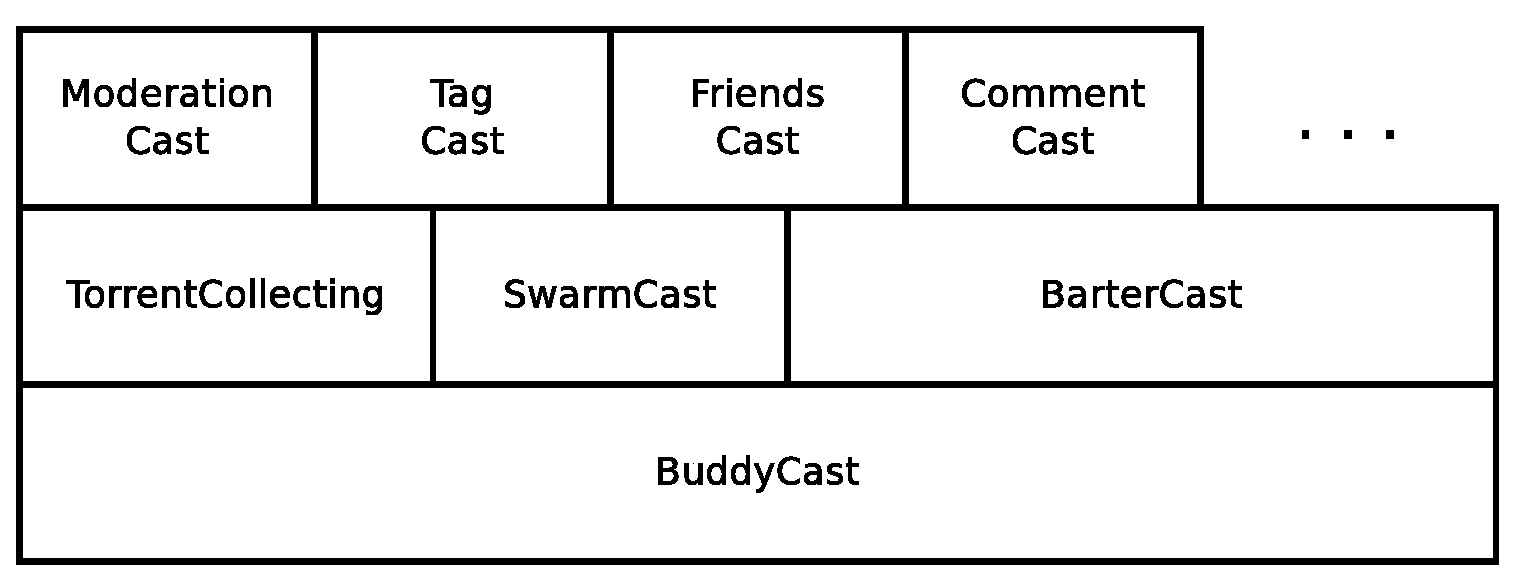
\includegraphics[scale=0.3]{relatedWork/figs/buddycast-stack.eps}}
	\caption{BuddyCast stack overview~\cite{pouwelse-buddycast}.}
	\label{fig:buddycast-stack}
\end{figure}

An epidemic protocol works in a very simple way relying on a receive-and-forward primitive.
Information is exchanged and forwarded between peers.
This is called gossiping.
BarterCasts gossips on the donation of upload bandwidth
and the consumption of download bandwidth by other peers.

BuddyCasts spreads information of other peers with initial messages.
This is done every 15 seconds, but a peer is only contacted every 4 hours to avoid contacting too often.
These messages contain a prefered content list, a list of peers with similair prefered content
and a list of random peers.
For each peer a public key, IP adress, port number and last seen timestamp is provided.
The peers with a similair preference are called taste buddies.
A format of the these messages can be seen in Figure \ref{fig:buddycast-format}.

\begin{figure}
	\centerline{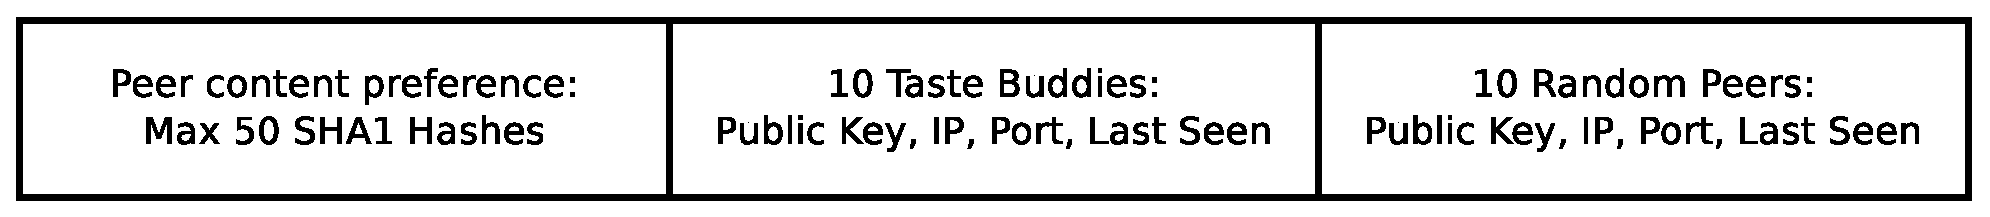
\includegraphics[scale=0.3]{relatedWork/figs/buddycast-format.eps}}
	\caption{Format of initial messages in BuddyCast~\cite{pouwelse-buddycast}.}
	\label{fig:buddycast-format}
\end{figure}

BuddyCasts uses several techniques to improve the peer selection efficiency.
Peer selection efficiency is the percentage of successfully delivered outgoing messages to peers.
This metric measures how well BuddyCasts selects peers on availablity and connectablity.
These are important because they determine how well BuddyCasts is able to handle with peer failure and exit.
Sending messages to an unavailable peer is a complete waste of resources.

The most obvious improvement that has been made is not to forward any offline peers.
BuddyCast maintains a live overlay
and continuously verify the online status of 10 random peers and 10 taste buddies.
The random peers are updated to ensure they are in fact random peers.

Peers can detect their own connectivity issues.
While they are able to connect outbound,
no incoming connections can be excepted.
These peers can improve the peer selection efficiency
by broadcasting that they are having connectivity problems
and instructing others to not gossip their identity.

Each peer collects information on how much other peers have downloaded and uploaded.
This information is signed and a barter record is created.
These barter records are forwarded to 10 peers.
A peer has a chance to be random peer or a taste buddy.
The records are forwarded by attaching them to BuddyCast messages.

The aggregrated information contains information about direct interactions with other peers,
but also information about interactions between other peers gossiped.
The information can be visualised using BarterBowser.
A screenshot can be seen in Figure \ref{fig:barterbrowser}.
The center contains the local peer.
Every circle contains peers for a certain degree.
The first circle from the centre contains peers that the local peer has direct interactions with.
The second circle contains peers that peers from the first circle has direct interactions with and so forth.
The figure shows how BarterCast accumulates data through other peers.

\begin{figure}
	\centerline{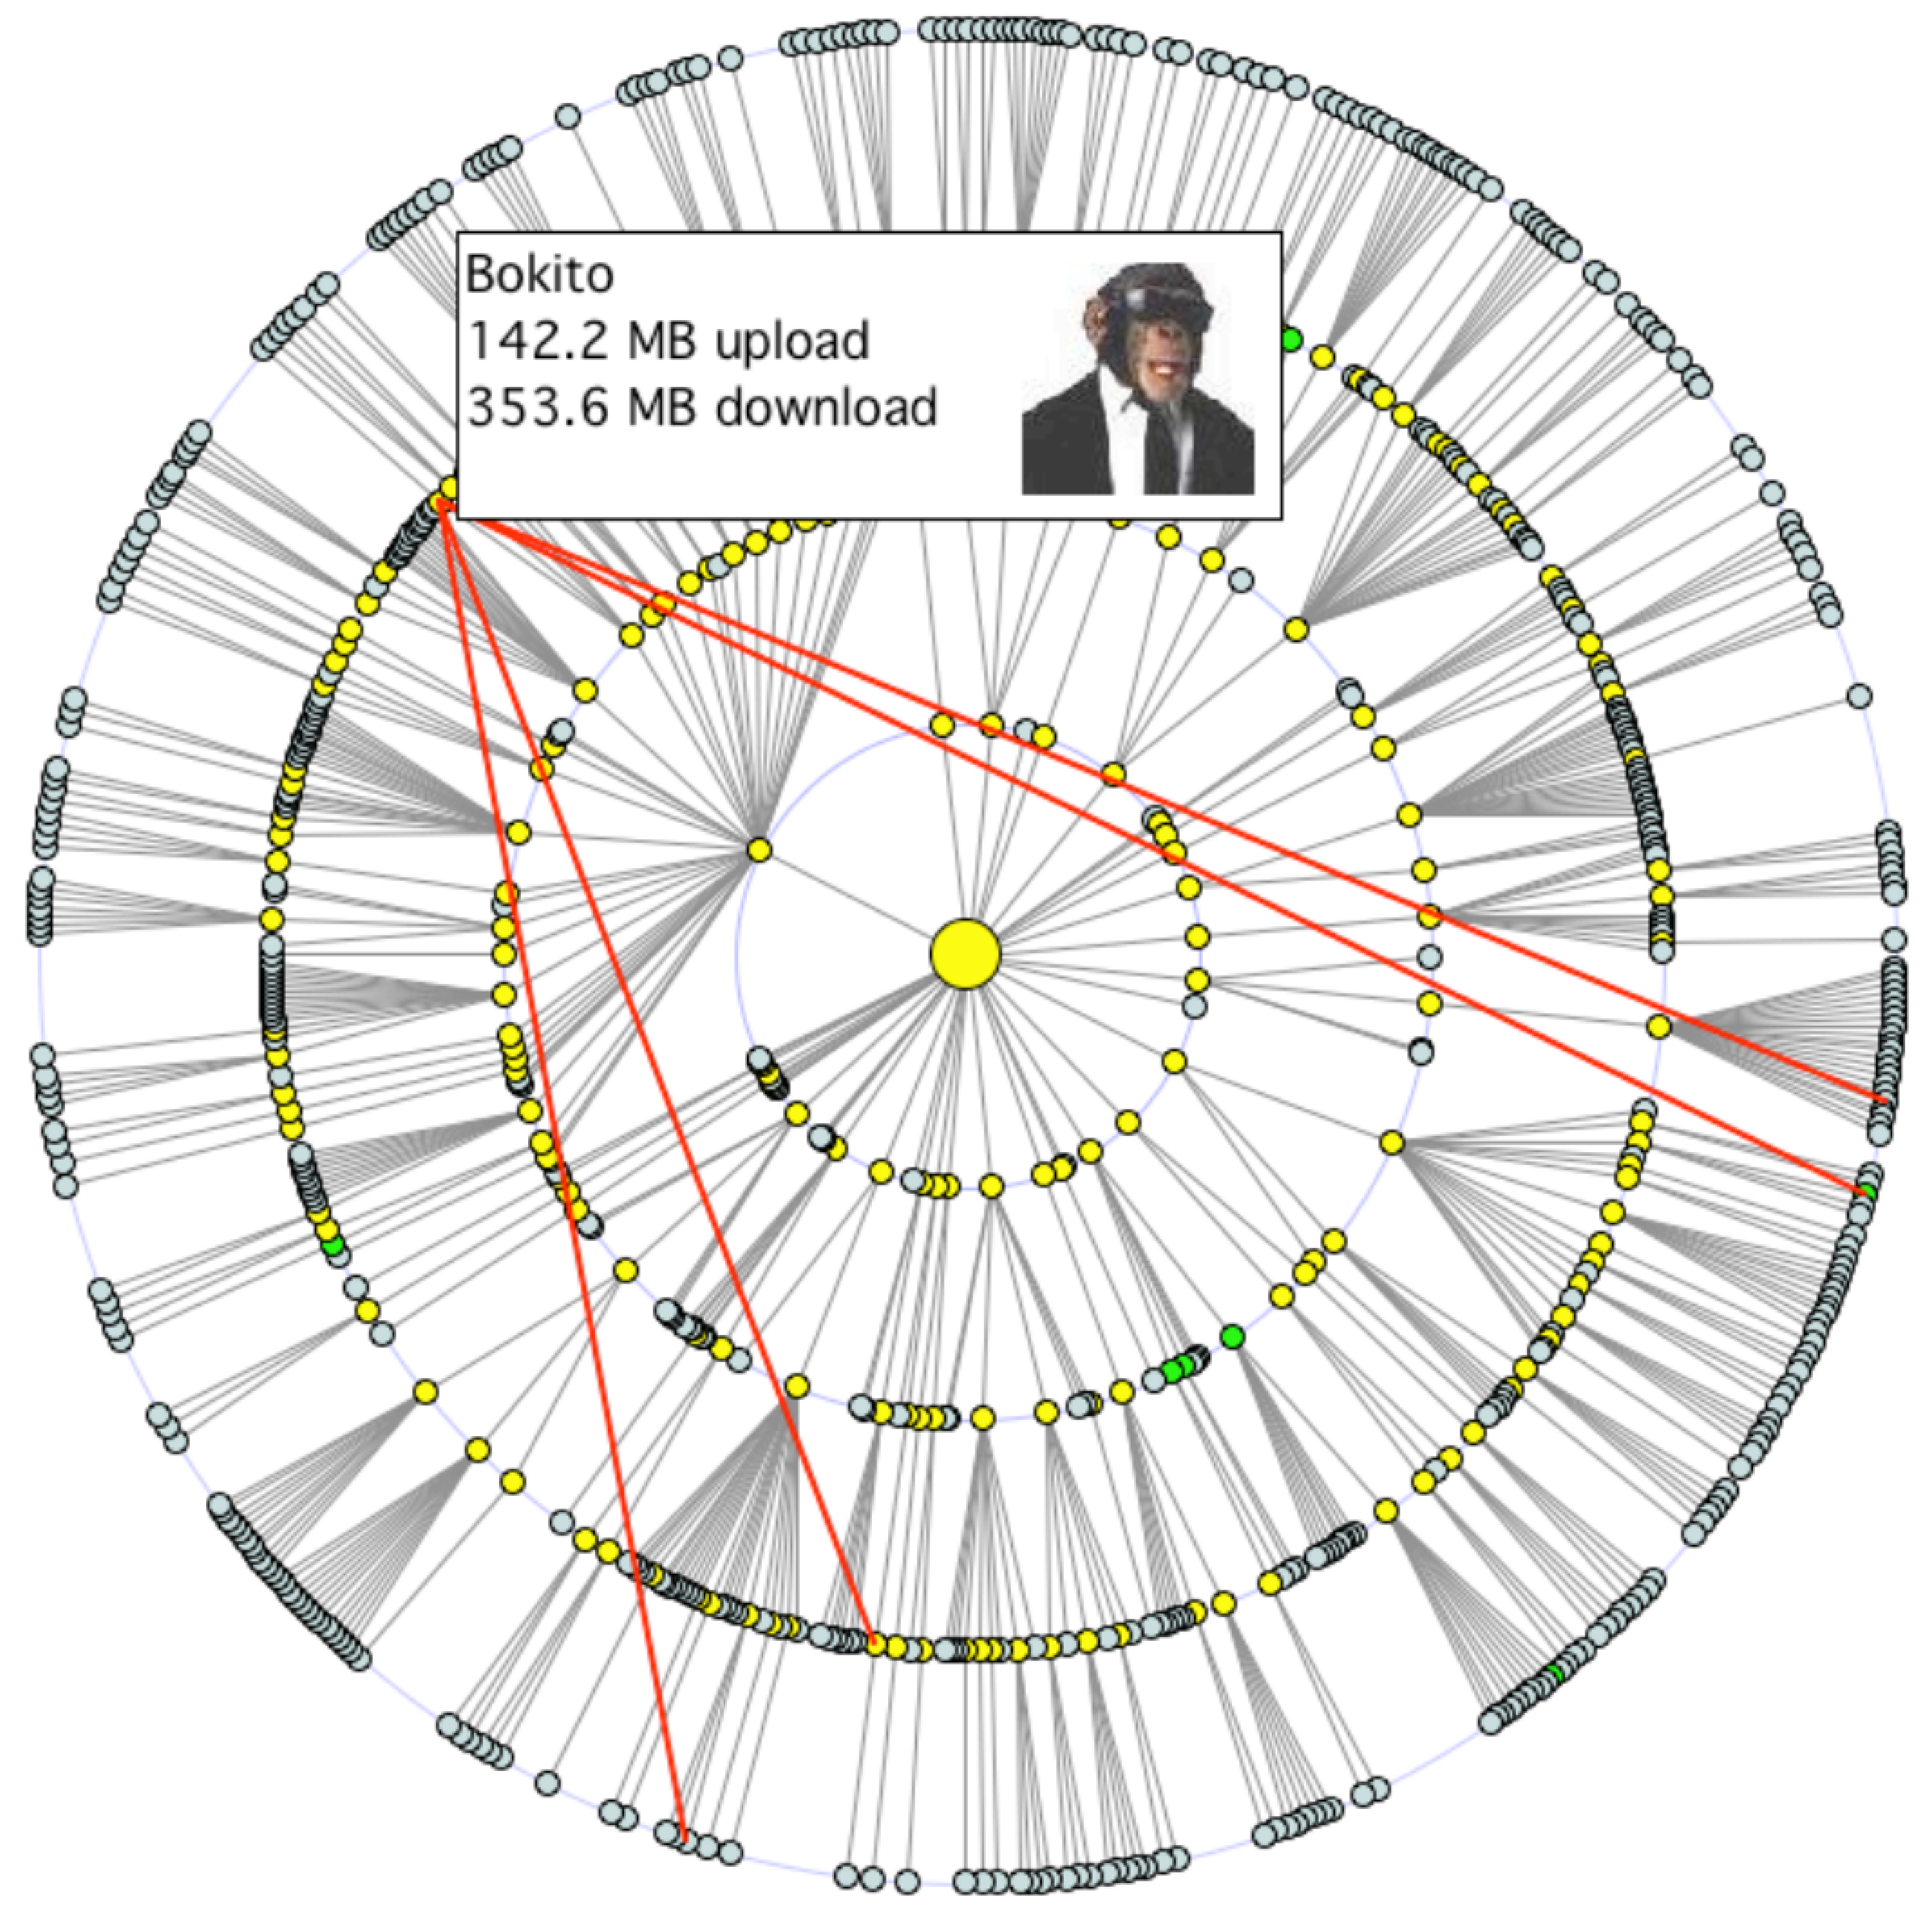
\includegraphics[width=0.8\textwidth]{relatedWork/figs/barterBrowser.eps}}
	\caption{A screenshot of BarterBrowser in 2008~\cite{pouwelse-buddycast}.}
	\label{fig:barterbrowser}
\end{figure}

The information can be used to in conjunction with the maxflow algorithm
to create a reputation metric~\cite{meulpolder-bartercast-paper}.
The reputation metric measures how well or how poorly a peer has helped the network.
The calculation takes into account that the difference between 0 and 100 MB is more significant
then between 1000 MB and 1100 MB.

The calculation is done without relying on a third party.
No authority verifies the validity of the received information.
Also there is no insurance that the information is complete.

Improvements have been done to improve the performance of BarterCast.
A bloom filter algorithm is implemented to decrease the amount of duplicate barter records
being sent to peers already having those records~\cite{logiotatidis-splash}.
Bloom filters can be used to quickly determine with some certainty
if a database contains records in limited space~\cite{broder-bloomfilter}.
The bloom filter protocol works in the following way:
\begin{enumerate}
    \item Peer $A$ creates a specific Bloom filter for peer $B$.
    \item Peer $A$ sends the Bloom filter to peer $B$.
    \item Peer $B$ checks every record in its database using the Bloom filter.
    \item Peer $B$ sends any missing record to peer $A$.
\end{enumerate}
The created bloom filters only contain relevant entries that have not yet been synchronized to peer $B$.
BarterCasts knows which entries are relevant by keeping track of the last synchronization point
and only using new barter records since that point.

\subsection{Limitation}
The main limitation of Bartercast is that the reputation is self reported.
This assumes the majority of nodes to be honest and to follow protocol.
Barter records are not signed by any one else.
So Barter records can be created by any malicious node without a limit.
There is no way to verify these records and enforce truthfulness.
Finally, there is no way to punish malicious nodes and therefore they are free to lie.



